\section{Abstract Translation Algorithm}
\label{sec:AbstractTranslation}

We propose to modify basic LALR-based algorithm of abstract parsing to solve the problem of abstract 
translation. The original parsing algorithm targeted to recognition, not translation, and it does not 
support semantics calculation. This fact allows to operate only with tokens type, not tokens values. 
It is possible to merge states like in GLR-algorithm\footnote{Generalized Left-to-right Rightmost 
derivation -- LR-based parsing algorithm for arbitrary (ambiguous) context-free grammars 
processing~\cite{Grune}.}. This way we can avoid problems with size of states set and parsing result.
If we want to translate input expression to another language then we should keep all information 
about tokens values. 

One of the possible solution of translation is abstract parsing algorithm with mechanism of stack 
splitting for semantic calculation support. It disallow to merge states and we should create new 
copies of stack on each branch in input graph and get exponential memory usage in worst case. 
Note that there is a big number of dynamic expressions which require exponential resources to 
analyze in the real world information systems. 

For example parser states for vertex $V_3$ in picture~\ref{pic4} should be equal for 2 input edges
but if we want to calculate semantics, then we get two different states because identifiers has 
different values.

\begin{figure}
    \begin{center}
        \includegraphics[width=9cm,height=1.1cm]{graphs/states_example.eps}
        \caption{Graph with states possible to merge}
        \label{pic4}
    \end{center}
\end{figure}

Queries which contains a huge number of branches is a big problem. The number of states is an 
exponential function of the Nnumber of branches because for each branch we should produce $n*k$ 
states where $n$ is a number of states in root of fork vertex and $k$ is a number of branches. 
One of the most frequent example of queries with big number of branches is \verb|select| query. 
Each of fields to select can be calculated with if-statement or case-statement. Example of such 
graph presented in picture~\ref{pic5}.

\begin{figure}
    \begin{center}
        \includegraphics[width=7.7cm,height=1.5cm]{graphs/big_res.eps}
        \caption{Graph which requires an exponential resources for translation}
        \label{pic5}
    \end{center}
\end{figure}

If we use only sequentially concatenated if-statements then the number of parsing trees is $2^n$ 
where $n$ is a number of if-statements (or number of branches). In the real-world systems we 
have faced the queries which contains more than 100 branches. Full forest calculation by naive 
adaptation of abstract parsing is impossible for such queries. The set of states to be processed
 minimization is an actual problem for real-world systems.

%\subsection{Optimization of the abstract translation algorithm}
%\label{sec:Optimizations}

We propose the following solution of forest size minimization problem. We have previously discussed 
that the result of translation is new values for all variables which were used for queries construction. 
It is sufficient to construct not the full forest but only the minimal set of trees such that after 
translation every variable gets new value.This way, we can process not all paths in the input graph 
but only minimal set which contains all edges. Note that we cannot calculate this set before parsing 
because we cannot be sure that every path produces syntax correct values. If some path contains 
error than the tree is not constructed and we lose information about variables. For example let
we try to process the graph presented in picture~\ref{pic6}.

\begin{figure}
    \begin{center}
        \includegraphics[width=4.8cm,height=1.2cm]{graphs/paths.eps}
        \caption{Graph for minimal paths set selection.}
        \label{pic6}
    \end{center}
\end{figure}

One possible set of paths which we can be calculated before syntax analysis is $\{(L_1; M_1); (L_2; M_2)\}$. 
But every path contains syntax errors and the result forest is empty instead of containing 2 trees. 
We should choose another set (for example $\{(L_1; M_2); (L_2; M_1)\}$) to get correct result. So, 
path calculation is iterative process. We should perform states filtering during syntax analysis 
for each vertex with multiple input edges. Let we describe steps of the process.

\begin{itemize}
    \item \textbf{Initial state.} Set of states for vertex is empty. 
    \item \textbf{Step.} For each step if the current vertex has multiple input edges then we should add new state to states set for current vertex if any of the next conditions is true.
    \begin{itemize}
        \item New state corresponds with path which contains edges which are not contained in any of paths corresponded with states in the currently processed set. 
        \item New state corresponds with parser state which is not presented in the currently processed set.
    \end{itemize}

\end{itemize}

\begin{comment}
Described algorithm pseudo code is presented below.
\begin{verbatim}
/*
V – list of input graph vertices in the topological order.
v_s – start vertex of input graph.
*/

let filterStates v =
    let groupedByParserState =
        v.States.GroupBy (fun state -> state.Item)

    v.States = Set.empty

    for group in groupedByParserState do
        /* Each state corresponds with path from v_s to v.
         Set of paths specify set of edges of graph E_s.
         We should construct minimal set of paths which
         contains all edges of E_s. The next greedy algorithm
         can be applied to solve this problem.
         1) Order paths by length ascent.
         2) While current path contains edges not in
         the result set add this path in the result set.*/
        let ordered = 
            group.OrderBy (fun s -> -1 * s.Path.Lenght)
        for s in ordered do
            if (s.Path contains edges which 
                not in any path from result set) 
            then v.States.Add s

for v in V do
    v.States <- … /*step of syntax analysis*/
    /*If input degree of the vertex v more 
      then 1 then try to filter states.*/
    if v.InEdges.Count > 1 then filterStates v

\end{verbatim}
\end{comment}

This way we can get states set which contains all parser states from input set but is not greater 
than it. Corresponded paths contains all possible edges in processed subgraph. Described algorithm
of filtration allows to increase performance of parsing by decreasing a number of parsing trees.
